\documentclass[11pt]{article}
%Gummi|061|=)

\usepackage{xcolor}
\usepackage{listings}
\usepackage{graphicx}


\title{\textbf{User Manual\linebreak Parametrized String Matching Implementation for Software Plagiarism Check}\footnote{Although the official name of this project is \emph{Parametrized String Matching Implementation for Software Plagiarism Check}, internally within the team we had code named it as the \textbf{\emph{CopyDog}}. Any reference to CopyDog in this or other documents shall be understood to as referring the same project only.} }
\author{ 		
        \vspace{ 2 mm}\\
		Supervised By : \textbf{Prof. Srinivasaraghavan G}\\
		\vspace {2mm}\\
		\textbf{Team} \\	
		amit.tomar \\
		(MT2013008) \\
		\vspace{ -1 mm}\\		
		siddhesh.dosi\\								     
		(MT2013150) \\		
		\vspace{ -1 mm}\\					
		srinivas.r.vaidya\\
		(MT2013152) \\
		\vspace{ -2 mm}\\		
		\textbf{@iiitb.org}}
		
\date{26 - July - 2014 \vspace {35 mm}}

\begin{document}

\maketitle

\vspace {85 mm}

\section{Launching the application}

If all the dependencies (mentioned later in the document) are met properly, application can be launched as follows :

\begin{enumerate}

\item Change the directory to the folder containing your application.

 \item Execute the command
 
\emph{ ./CopyDog }

Change the permissions using \emph{chmod} command, in case you get permissions related errors.
 	
\item You can also execute it by double clicking using a GUI.

\end{enumerate}

\section{Using the Application}

CopyDog works in two mode of operations. Using one option you can select all the files in the selected folder, with the selected language extension, automatically. In the second option, you can select the files manually to check them for plagiarism. In the \emph{Startup Screen}, you can select the language you want to check plagiarism on, and the minimum number of characters that should be considered for any plagiarism related case. Then you can click on of the following options :

\vspace{ 3 mm} 

\noindent \textbf{Select all files in the folder}

\vspace{ 3 mm} 

\noindent Clicking on this option, opens up a folder browser which allows to select all the files in that folder, of the extension corresponding to the language specified by you, and generates the plagiarism related information.

\vspace{ 3 mm} 

\noindent \textbf{Select files manually}

\vspace{ 3 mm} 

\noindent Clicking on this option, opens up a file browser which allows to select files manually in that folder, and generates the plagiarism related information.

\vspace{ 3 mm} 

\noindent \textbf{Export and Exit}

\vspace{ 3 mm} 

\noindent CopyDog also provides an efficient way to save the plagiarism related information in persistence. You can simply click on the save and exit button. CopyDog will save the information in your current working directory with name:

\emph{CopyDogPlagiarismInformation\_[TimeStamp]}. 

\begin{figure}[p]
    \centering
    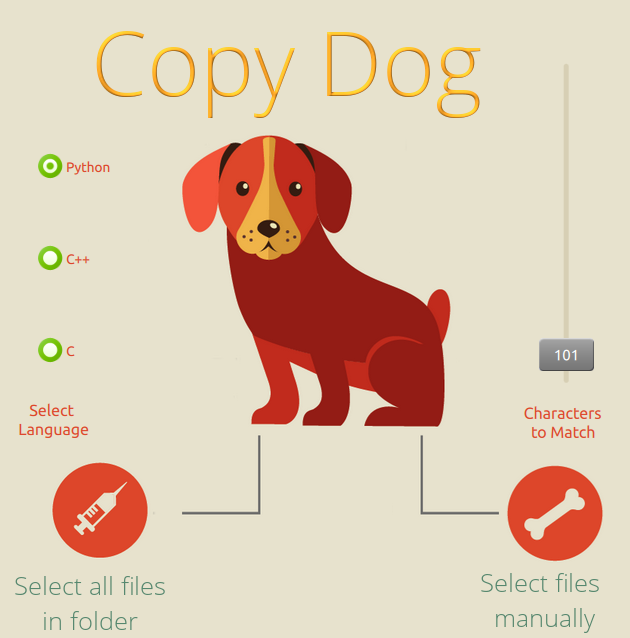
\includegraphics[scale=.6]{MainScreen.png}
    \caption{Main Screen of CopyDog}
\end{figure}

\begin{figure}[p]
    \centering
    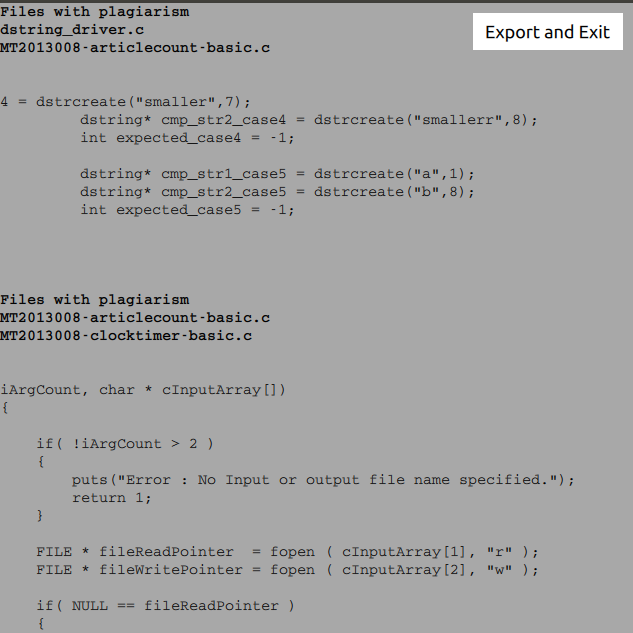
\includegraphics[scale=.5]{PlagInfoScreen.png}
    \caption{Screen showing Plagiarim information}
\end{figure}


\section {Dependencies and Build} 

CopyDog has been built using Qt-5.3. Though there should not be problems with any version of Qt greater than version 5.0. The uploaded built version is for 32-bit Intel platform. Any other platform will require a rebuild of the project. \emph{Src} folder in the code contains a \emph{.pro} of Qt, which can the opened up using the Qt-Creator IDE for editing/compilation purposes. In case the IDE is not available, the Makefile present in the \emph{Build} folder can also be used for a re-build. Try doing a clean-build to avoid any mismatch in the library version of the obj files already present in the Build folder. Python version 2.7 has been used for the Python code.

\vspace{3mm}
\noindent Following files whould be present in the same folder as the  executable : 

\begin{enumerate}

\item CopyDog.png

 \item MainScreen.png
 
  \item slider.png
  	
\item radioChecked.png

\item radioUnchecked.png

\item main.qml

\item PythonParser.py

\item Unparse.py

\end{enumerate}

\vspace{ 3 mm}


\section{References}
 
Following sources were referred before writing this documents to get the basic understanding of Kernel development process and approximate time it might require:
 
\vspace {3 mm}

 
 \begin{enumerate}
 
 \item  
 
 \textbf{ Images}
 
Dog image present on the home screen has been taken from the work of Marina Zlochin. (\emph{Usage request for this image is still pending with her.})
 
 {https://www.behance.net/ma\_rish}
 
 \vspace {5 mm}
 

 
 \item  \textbf{ Python Code} 
 
 For converting the Abstarct Synax Tree structures of Python code to the normal source code of Python, we have used an \emph{Unparser} from this site :
 
 { http://svn.python.org/projects/python/trunk/Demo/parser/unparse.py}
 

 

 
 
 \end{enumerate} 

\end{document}
